\documentclass[11pt,oneside,notitlepage]{book}

\RequirePackage{lineno}
\usepackage{import}
\usepackage{csquotes}
\usepackage{titlesec}
\usepackage{enumitem}
\usepackage{amssymb, amsmath}
\usepackage{mathpazo}
\usepackage{float,graphicx}
\graphicspath{{./figs}}
\usepackage[figuresright]{rotating}
\usepackage[usenames,dvipsnames]{color}
\usepackage{microtype}
\usepackage{tabulary}
\usepackage{booktabs,multirow,dcolumn,bigdelim}
\newcommand{\otoprule}{\midrule[\heavyrulewidth]}
\usepackage{xr-hyper}
\usepackage[pdftex,plainpages=false,pdfpagelabels,backref,pdfborder={0 0 0}]{hyperref}
%\externaldocument{ReviewResponses/DOE_review_responses_11202014}
\usepackage{url}
\usepackage[toc,page,titletoc]{appendix}
\usepackage{afterpage}
\usepackage[font=small,labelfont=bf]{caption}
\setlength\captionmargin{15pt}
\usepackage[scaled]{helvet}
\usepackage{sectsty}
\allsectionsfont{\normalfont\sffamily}
\usepackage{titletoc}
\titlecontents{chapter}
  [1.5em]
  {\linespread{0.9}\normalfont\sffamily\bfseries}
  {\contentslabel{1em}} 
  {\hspace*{-2.3em}} 
  {\mdseries\titlerule*[1pc]{.}\contentspage} 
\titlecontents{section}
  [3.5em]
  {\linespread{0.9}\normalfont\sffamily}
  {\contentslabel{2.3em}} 
  {\hspace*{-2.3em}} 
  {\titlerule*[1pc]{.}\contentspage} 
\titlecontents{subsection}
  [4.5em]
  {\linespread{0.9}\normalfont\sffamily}
  {\contentslabel{2.3em}} 
  {\hspace*{-2.3em}} 
  {\titlerule*[1pc]{.}\contentspage} 
\titlecontents{subsubsection}
  [5.5em]
  {\linespread{0.9}\normalfont\sffamily}
  {\contentslabel{2.3em}} 
  {\hspace*{-2.3em}} 
  {\titlerule*[1pc]{.}\contentspage} 
\tolerance = 10000

\usepackage[text={6.5in,8.75in},headheight=15pt,centering]{geometry}
\usepackage{xspace}

\DeclareGraphicsExtensions{.pdf,.png}
\newcommand{\filenamedot}{.}
\setlength{\parindent}{0.0in}
\setlength{\parskip}{0.1in}
\renewcommand{\topfraction} {0.9}
\renewcommand{\bottomfraction} {0.9}
\renewcommand{\textfraction} {0.1}
\renewcommand{\floatpagefraction} {0.8}

\usepackage{fancyhdr}
\pagestyle{fancy}
\renewcommand{\chaptermark}[1]{\markboth{#1}{}}
\renewcommand{\sectionmark}[1]{\markright{#1}{}}
\fancyhead{} % clear all header fields 
\fancyhead[RO,LE]{\sffamily \rightmark}
\fancyhead[LO,RE]{\sffamily \leftmark}
\fancyfoot{} % clear all footer fields 
\fancyfoot[RO,LE]{\sffamily \thepage}
\renewcommand{\headrulewidth}{0pt} 
\fancypagestyle{plain}{%
  \fancyhf{}
  \fancyfoot[RO,LE]{\sffamily \thepage}
}

\usepackage{eurosym}
\usepackage{xcolor}
\usepackage{framed}
\colorlet{shadecolor}{blue!10}

\setcounter{secnumdepth}{2}
\setcounter{tocdepth}{1}

\newcommand{\lyxdot}{.}
\usepackage{subfig}

\setlength\fboxsep{0pt}
\setlength\fboxrule{0.5pt}
\title{sPHENIX baseline scope}
\begin{document} 

%\linenumbers

\frontmatter

\pagestyle{empty}
\newcommand{\hic}{\mbox{$A$$+$$A$}\xspace}
\newcommand{\pA}{\mbox{$p$$+$$A$}\xspace}
\newcommand{\AuAu}{\mbox{Au$+$Au}\xspace}
\newcommand{\auau}{\mbox{Au$+$Au}\xspace} 
\newcommand{\raa}{\mbox{$R_{AA}$}\xspace}
\newcommand{\pbpb}{\mbox{Pb$+$Pb}\xspace} \newcommand
{\pdau}{\mbox{$p(d)$$+$Au}\xspace} \newcommand
{\aj}{\mbox{$A_J$}\xspace} \newcommand {\pp}{\mbox{$p$$+$$p$}\xspace}
\newcommand {\ppbar}{\mbox{$p$$+$$\overline{p}$}\xspace}
\newcommand{\pT}{\mbox{${p_T}$}\xspace}
\newcommand{\jpsi}{\mbox{$J/\psi$}}
\newcommand{\sqrtsnn}{\mbox{$\sqrt{s_{\scriptscriptstyle NN}}$}}
\newcommand{\npart}{$N_\mathrm{part}$}
\newcommand{\ncoll}{$N_\mathrm{coll}$}
\newcommand{\qgp}{\mbox{quark-gluon plasma}\xspace}
\newcommand{\jt}{\mbox{$J_T$}} \newcommand{\qhat}{\mbox{$\hat{q}$}}
\newcommand{\Qsqr}{\mbox{$Q^2$}} \newcommand{\CuCu}{\mbox{Cu$+$Cu}}
\newcommand{\PbPb}{\mbox{Pb$+$Pb}} \newcommand{\pPb}{\mbox{$p$$+$Pb}}
\newcommand{\gjet}{\mbox{$\gamma$-jet}}
\newcommand{\Qmax}{\mbox{$Q_{\max}$}} \newcommand{\ET}{\mbox{$E_T$}}
\newcommand{\Et}{\mbox{$E_T$}} \newcommand{\kt}{\mbox{$k_T$}}
\newcommand{\RAA}{\mbox{$R_{AA}$}\xspace} \newcommand{\IAA}{\mbox{$I_{AA}$}}
\newcommand{\pt}{\mbox{${p_T}$}\xspace}
\newcommand{\highpt}{high-${\rm p_{_{T}}}$}
\newcommand{\lessim}{{\stackrel{<}{\sim}}} \newcommand{\eqnpt}{p_T}
\newcommand{\eA}{\mbox{$e-{\rm A}$}}
\newcommand{\dAu}{\mbox{$d$$+$Au}\xspace}
\newcommand{\pAu}{\mbox{$p$$+$Au}\xspace}
\newcommand{\pau}{\mbox{$p$$+$Au}\xspace}
\newcommand{\GeVSQ}{\mbox{${\rm GeV}^2$}}
\newcommand{\fastjet}{\mbox{\sc FastJet}\xspace}
\newcommand{\geant}{\mbox{\sc Geant4}\xspace}
\newcommand{\antikt}{\mbox{anti-$k_T$}\xspace}
\newcommand{\pythia}{\mbox{\sc Pythia}\xspace}
\newcommand{\rapgap}{\mbox{\sc Rapgap}\xspace}
\newcommand{\milou}{\mbox{\sc Milou}\xspace}
\newcommand{\pyquen}{\mbox{\sc Pyquen}\xspace}
\newcommand{\hijing}{\mbox{\sc Hijing}\xspace}
\newcommand{\roofit}{\mbox{\sc RooFit}\xspace}
\newcommand{\roounfold}{\mbox{\sc RooUnfold}\xspace}
\newcommand{\beetle}{\mbox{\sc Beetle}\xspace}
\newcommand{\gj}{\mbox{$\gamma$+jet}\xspace}
\newcommand{\gh}{\mbox{$\gamma$+hadron}\xspace}
\newcommand{\martinimusic}{\mbox{\sc Martini+Music}\xspace}
\newcommand{\martini}{\mbox{\sc Martini}\xspace}
\newcommand{\music}{\mbox{\sc Music}\xspace}
\newcommand{\Ephenix}{Electron-Ion Collider (EIC) detector built
  around the BaBar magnet and sPHENIX calorimetry\xspace}
\newcommand{\ephenix}{EIC detector built around the BaBar magnet and
  sPHENIX calorimetry\xspace} 
\newcommand{\refdesign}{reference design\xspace}
\newcommand{\refconfig}{reference configuration\xspace}
\newcommand{\dijet}{\mbox{dijet}\xspace}
\newcommand{\fake}{\mbox{fake}\xspace}
\newcommand{\fast}{\mbox{fast}\xspace}
\newcommand{\veryfast}{\mbox{very fast}\xspace}
\newcommand{\epem}{\mbox{$e^+e^-$}\xspace}
\newcommand{\onewidth}{0.6\linewidth}
\newcommand{\twowidth}{0.48\linewidth}
\newcommand{\threewidth}{0.32\linewidth}

\newcommand{\egoing}{\mbox{electron-going}\xspace}
\newcommand{\hgoing}{\mbox{hadron-going}\xspace}
\newcommand{\egodir}{electron-going direction\xspace}
\newcommand{\hgodir}{hadron-going direction\xspace}

\renewcommand*\familydefault{\sfdefault}
{\sffamily
\vfill
\vspace{4cm}
\begin{figure}[H]
  \begin{center}
    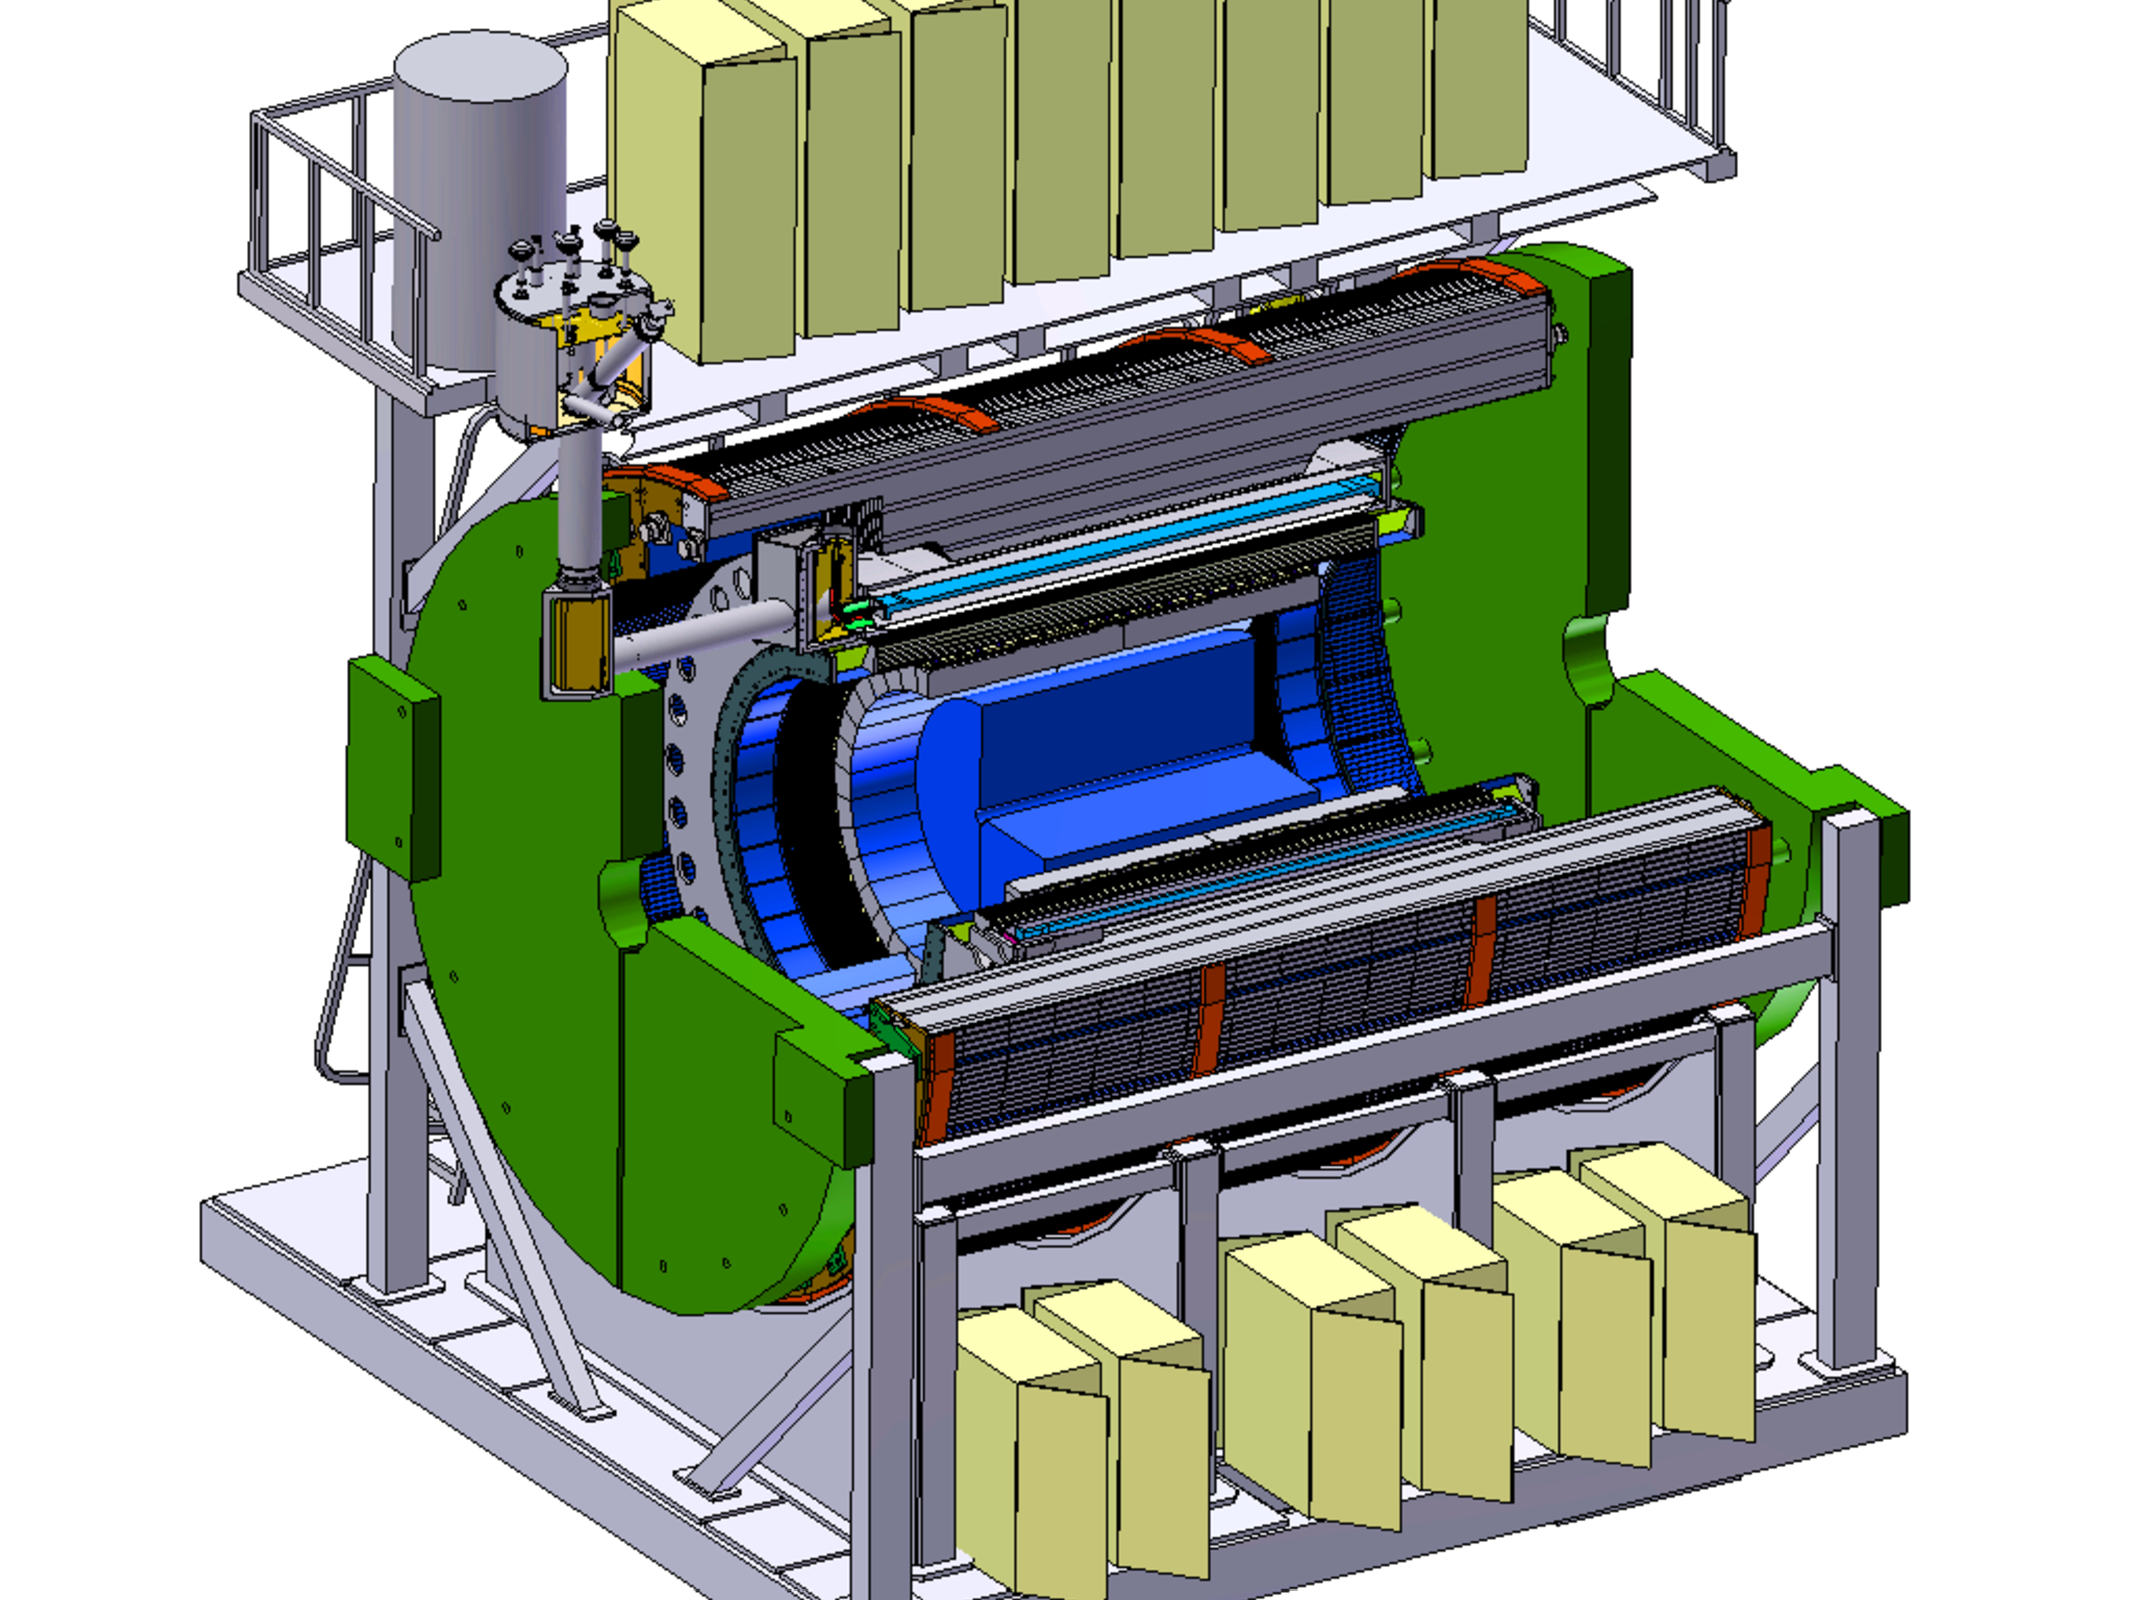
\includegraphics[width=\linewidth]{figs/sPHENIX}
  \end{center}
\end{figure}

\begin{center}
  \LARGE
  \vskip 2 em
  Addressing the Baseline Scope Charge\\
  \vskip 4 em
  The sPHENIX Collaboration \\
  May 31, 2016 \\
\end{center}

\vspace{2cm}

\begin{figure}[H]
  \begin{center}
    %\includegraphics[width=0.7\linewidth]{figs/cover}
  \end{center}
\end{figure}
}


\vfill
\renewcommand*\familydefault{\rmdefault}


\cleardoublepage
\pagestyle{fancy}
\section*{Executive Summary}
\label{executive_summary}
\setcounter{page}{1}

\nocite{*}

In this document the sPHENIX collaboration answers a charge~(see
Appendix~\ref{charge}) from BNL ALD Berndt Mueller to develop
a baseline design scope that provides a compelling phsyics program
within the constraints of possible DOE funding redirected from 
RHIC operations. The document describes a reference design aimed
at a compelling program focussed on three science drivers: jet structure,
heavy-flavor jet production and $\Upsilon$ spectroscopy. We then
provide a comprehensive list of re-scoping options for each
of the main subdetector systems, and describe the associated
cost savings, the engineering and schedule impact and impact on 
key performane measures related to the three science 
drivers. Based on these criteria, we develop examples of 
rank-ordered lists of re-scoping options including the 
cumulative cost-savings and science impact.




\cleardoublepage

\resetlinenumber

%\tableofcontents
\cleardoublepage

\mainmatter

\renewcommand{\thepage}{\arabic{page}}
\setcounter{chapter}{0}

\setcounter{page}{1}

\chapter*{Overview}
\label{configurations}
\setcounter{page}{1}

\section{Introduction}
In this document the sPHENIX collaboration answers a charge~(see
Appendix~\ref{charge}) from BNL ALD Berndt Mueller to develop
a baseline design scope that provides a compelling phsyics program
within the constraints of possible DOE funding redirected from 
RHIC operations. The document describes a reference design aimed
at a compelling program focussed on three science drivers: jet structure,
heavy-flavor jet production and $\Upsilon$ spectroscopy. We then
provide a comprehensive list of re-scoping options relative 
to the reference design for each
of the main subdetector systems, and describe the associated
cost savings, the engineering and schedule impact and impact on 
key performane measures related to the three science 
drivers. Based on these criteria, we develop examples of 
rank-ordered lists of re-scoping options including the 
cumulative cost-savings and science impact.

The total amount of redirected DOE funds available is quoted as \$75M in FY16 dollars.
Based on discussions between ALD, project and collaboration, the charge can
however more narrowly interpreted as aiming at a reduction in discretionary M\&S costs 
by \$4M in FY16 dollars compared to the detector design described
in the 2015 Director's Cost and Schedule review. In this document we will
therefore exclusively focus on these M\&S savings, excluding non-discretionary 
infrastructure items such as cryogenics, magnet, central pedestal and flux doors.


\section{Outer HCal}
\subsection{Thinned Outer HCal}
\label{ohcal_thin}

\textbf{Cost delta: -\$0.4M}

We investigated reducing the thickness of the outer HCal by 20~cm, or
approxiately one nuclear interaction length.  The thickness of the
outer HCal in the pCDR design is 86.5~cm.  Several possible effects
were investigated through full \geant simulations of the calorimeter
response.  It should be noted that the calorimeter simulations have
recently been compared to data from the FNAL test beam and have been
found to reproduce the measured response quite well.  We looked at the
effect of thinning on the jet energy response, high-$z$ fragmentation
functions.

From a physics perspective, the effect of thinning the outer HCal by
this amount seems to be moderate, and considered by itself, a thinner
outer HCal would still enable the core elements of the sphenix physics
program to be carried out.

From the perspective of the project, the effect of this modification
would be extremely significant.  The outer HCal is the structural
backbone of the sPHENIX structure.  Reducing the radial thickness
significantly reduces the ability of the outer HCal to support the
detector.  The finite element analysis would need to be redone, and
the tilt angle of the steel plates reanalyzed and likely changed. The
prototyping and test beam would have to be redone, delaying plans to
build a full scale mechanical prototype.  The inner HCal will need
some redesign due to the changes in the EMCal, as the $\phi$
segmentation of the two calorimeters should match for mechanical
reasons.  This option sets the outer HCal engineering back as much as
twelve months and requires R\&D be redone.

In the nominal design, the $5.5 \lambda$ total depth of the
calorimeter stack (at $\eta = 0$) is distributed as $1 \lambda$
(EMCal), $1 \lambda$ (inner HCal), and $3.5 \lambda$.  If the outer
HCal is reduced to $2.5 \lambda$, one has to consider the effects if
one or more of the other calorimeters in the stack is also modified.
If the inner HCal is not installed, the depth of the calorimeter stack
is reduced by an additional $1 \lambda$ over the whole acceptance,
falling to $2.5 \lambda$ at midrapidity.  If the EMCal acceptance is
cut to $|\eta| < 0.7$, the thickness of the calorimeter stack in the
range $0.7 < \eta < 1.1$ becomes thinner by $1 \lambda$, but the
effect in that range (aside from the lack of EMCal coverage) is
moderated by the increasing thickness of the calorimeters along lines
of constant $\eta$ due to their rectangular profile.



\chapter*{Shortened HCal}
\label{ohcal_short}

\section*{Inner HCal}
\label{ihcal}

We have considered not building and installing the inner HCal.  One
positive aspect is that by not building a detector, one saves the full
set of costs associated with engineering, prototyping and producing
the detector, not just a fraction of the production costs as would be
saved by building a fraction of the final detector.  The lack of an
active absorber between the outer radius of the EMCal and the cryostat
has pronounced effect on the science capabilities of sPHENIX. The jet
energy response is worsened by removing a full interaction length of
absorber, an effect that is amplified compared to naive expectation
because the volume normally occupied by the inner HCal is in a
1.5~tesla magnetic field.  The lower momentum components of showers
that initiate in the EMCal can be strongly bent in the absorber-free
space before the cryostat.  These particles can also curl around and
strike additional EMCal towers.  Because of these effects, the
colaboration strongly disfavors removing the inner HCal.

From a project perspective, the inner HCal is one of the subsystems
that has the potential to involve non-BNL machine shops.  In
particular, the shop capabilities of some collaborating sPHENIX
Universities could allow them to take a significant role in the
machining and construction of inner HCal modules.  Deciding not to
build this detector would reinforce a view that sPHENIX is essentially
a BNL-only project.

\section{EMCal}

The EMCal accounts for a significant portion of the M\&S budget.  It
also enables the key $\Upsilon$ and direct $\gamma$ and $\gamma+$jet
capabilities of sPHENIX.  

\subsection{Reduction in EMCal Segmentation}
\label{emcal_ganging}
\label{emcal_segmentation}

\textbf{Cost delta: -\$1.7M}

We have considered two options to reduce the electronics cost
associated with the EMCal by reducing the segmentation.  One is
ganging together groups of 2x2 towers in the reference configuration
tower size ($\Delta\eta\times\Delta\phi = 0.024\times0.024$, leading
to an effective segmentation of $0.048 \times 0.048$) and the other is
to make a permanent reduction in the EMCal granularity by making the
towers bigger (one such configuration could be $0.033 \times 0.028$ in
$\Delta \phi x \Delta \eta$), reducing the number of towers by about
38\%. Both options for reducing the segmentation are estimated to
yield approximately the same cost savings.

Ganging together towers means that the R\&D done to date --- both on
production aspects as well as performance in the test beam --- remains
valid.  It does introduce a ``mortgage'' in which the collaboration
would try to identify funds to buy the additional electronics needed
to allow towers be read out individually.

Reducing the EMCal granularity via larger towers would reduce the cost
of the readout electronics, but would likely require increasing the
number of SiPMs per tower to preserve the light collection
uniformity. An advantage of the second option is that this would
provide a finer segmentation than the ganging option, however it would
not allow the reference configuration segmentation to be recovered.
Because this reduced granularity would be a permanent change, it does
not result in a mortgage.

The EMCal R\&D to this point has focused on the production of towers
of the $0.024\times 0.024$ size in the reference configuration.
Increasing the tower size introduces potential production issues in
the tower construction and performance. Additional R\&D will need to
be done to determine if larger towers can be made as efficiently and
uniformly as in the reference configuration and that the light can be
collected from larger area lowers with sufficient uniformity.  If this
option is pursued we would need to pursue R\&D on the larger size
towers to address the concerns described above and based on those
finding to decide which option provides the most feasible construction
option.  This R\&D would delay the overall EMCal schedule by
approximately six months and might require additional prototyping
beyond that which is currently in the schedule.

\subsection{EMCal Coarsened Segmentation}
\label{emcal_segmentation}

\textbf{Cost delta: $-\$1.8M$}

We have investigated reducing the number EMCal towers from
$256\times96=24576$ ($\Delta\eta\times\Delta\phi = 0.024 \times 0.024$) to
$192\times80 = 15360$ ($\Delta\eta\times\Delta\phi = 0.033 \times 0.028$) a
reduction of tower numbers by 37.5\%.  
\chapter*{TPC}
\label{tpc}

\section{MAPS}
\label{maps}

\section{DAQ/Trigger}
\label{daq}

\textbf{Cost delta: -\$1.5M}

The costs associated with the DAQ and Trigger are an area where
significant reductions are achievable.  Although we think the
\$0.5M trigger detector is a suitable target for a non-DOE, possibly
non-US, contribution, for the purposes of answering this charge, we do
not assume that that will happen.  Each of the RHIC experiments has
built trigger detectors that would suit the needs of sPHENIX, and some
of these detectors, such as the trigger detector used by PHOBOS, are
currently unused and available.  We would repurpose one of these
detectors for use in sPHENIX and reduce the M\&S costs accordingly.

We would reuse the infrastructure currently in place in the PHENIX
counting house, consisting of data collection modules (DCMIIs),
subevent buffers (SEBs), assembly and trigger processors (ATPs), a
high throughput networking switch and several racks of computers.
Some amount of new equipment would be needed, such as new level-1 and
global trigger boards.  There is some risk associated with this
approach, as it means, absent funds to renew th computing
infrastructure, starting a new experiment with computing that will be
by then several years old.





\cleardoublepage

\appendix

\chapter{Cost, engineering and schedule impact}
\label{cha:engineering}
\section{Outer HCal}
\subsection{Thinned Outer HCal}
\label{ohcal_thin}

\textbf{Cost delta: -\$0.4M}

We investigated reducing the thickness of the outer HCal by 20~cm, or
approxiately one nuclear interaction length.  The thickness of the
outer HCal in the pCDR design is 86.5~cm.  Several possible effects
were investigated through full \geant simulations of the calorimeter
response.  It should be noted that the calorimeter simulations have
recently been compared to data from the FNAL test beam and have been
found to reproduce the measured response quite well.  We looked at the
effect of thinning on the jet energy response, high-$z$ fragmentation
functions.

From a physics perspective, the effect of thinning the outer HCal by
this amount seems to be moderate, and considered by itself, a thinner
outer HCal would still enable the core elements of the sphenix physics
program to be carried out.

From the perspective of the project, the effect of this modification
would be extremely significant.  The outer HCal is the structural
backbone of the sPHENIX structure.  Reducing the radial thickness
significantly reduces the ability of the outer HCal to support the
detector.  The finite element analysis would need to be redone, and
the tilt angle of the steel plates reanalyzed and likely changed. The
prototyping and test beam would have to be redone, delaying plans to
build a full scale mechanical prototype.  The inner HCal will need
some redesign due to the changes in the EMCal, as the $\phi$
segmentation of the two calorimeters should match for mechanical
reasons.  This option sets the outer HCal engineering back as much as
twelve months and requires R\&D be redone.

In the nominal design, the $5.5 \lambda$ total depth of the
calorimeter stack (at $\eta = 0$) is distributed as $1 \lambda$
(EMCal), $1 \lambda$ (inner HCal), and $3.5 \lambda$.  If the outer
HCal is reduced to $2.5 \lambda$, one has to consider the effects if
one or more of the other calorimeters in the stack is also modified.
If the inner HCal is not installed, the depth of the calorimeter stack
is reduced by an additional $1 \lambda$ over the whole acceptance,
falling to $2.5 \lambda$ at midrapidity.  If the EMCal acceptance is
cut to $|\eta| < 0.7$, the thickness of the calorimeter stack in the
range $0.7 < \eta < 1.1$ becomes thinner by $1 \lambda$, but the
effect in that range (aside from the lack of EMCal coverage) is
moderated by the increasing thickness of the calorimeters along lines
of constant $\eta$ due to their rectangular profile.



\chapter*{Shortened HCal}
\label{ohcal_short}

\section*{Inner HCal}
\label{ihcal}

We have considered not building and installing the inner HCal.  One
positive aspect is that by not building a detector, one saves the full
set of costs associated with engineering, prototyping and producing
the detector, not just a fraction of the production costs as would be
saved by building a fraction of the final detector.  The lack of an
active absorber between the outer radius of the EMCal and the cryostat
has pronounced effect on the science capabilities of sPHENIX. The jet
energy response is worsened by removing a full interaction length of
absorber, an effect that is amplified compared to naive expectation
because the volume normally occupied by the inner HCal is in a
1.5~tesla magnetic field.  The lower momentum components of showers
that initiate in the EMCal can be strongly bent in the absorber-free
space before the cryostat.  These particles can also curl around and
strike additional EMCal towers.  Because of these effects, the
colaboration strongly disfavors removing the inner HCal.

From a project perspective, the inner HCal is one of the subsystems
that has the potential to involve non-BNL machine shops.  In
particular, the shop capabilities of some collaborating sPHENIX
Universities could allow them to take a significant role in the
machining and construction of inner HCal modules.  Deciding not to
build this detector would reinforce a view that sPHENIX is essentially
a BNL-only project.

\section{EMCal}

The EMCal accounts for a significant portion of the M\&S budget.  It
also enables the key $\Upsilon$ and direct $\gamma$ and $\gamma+$jet
capabilities of sPHENIX.  

\subsection{Reduction in EMCal Segmentation}
\label{emcal_ganging}
\label{emcal_segmentation}

\textbf{Cost delta: -\$1.7M}

We have considered two options to reduce the electronics cost
associated with the EMCal by reducing the segmentation.  One is
ganging together groups of 2x2 towers in the reference configuration
tower size ($\Delta\eta\times\Delta\phi = 0.024\times0.024$, leading
to an effective segmentation of $0.048 \times 0.048$) and the other is
to make a permanent reduction in the EMCal granularity by making the
towers bigger (one such configuration could be $0.033 \times 0.028$ in
$\Delta \phi x \Delta \eta$), reducing the number of towers by about
38\%. Both options for reducing the segmentation are estimated to
yield approximately the same cost savings.

Ganging together towers means that the R\&D done to date --- both on
production aspects as well as performance in the test beam --- remains
valid.  It does introduce a ``mortgage'' in which the collaboration
would try to identify funds to buy the additional electronics needed
to allow towers be read out individually.

Reducing the EMCal granularity via larger towers would reduce the cost
of the readout electronics, but would likely require increasing the
number of SiPMs per tower to preserve the light collection
uniformity. An advantage of the second option is that this would
provide a finer segmentation than the ganging option, however it would
not allow the reference configuration segmentation to be recovered.
Because this reduced granularity would be a permanent change, it does
not result in a mortgage.

The EMCal R\&D to this point has focused on the production of towers
of the $0.024\times 0.024$ size in the reference configuration.
Increasing the tower size introduces potential production issues in
the tower construction and performance. Additional R\&D will need to
be done to determine if larger towers can be made as efficiently and
uniformly as in the reference configuration and that the light can be
collected from larger area lowers with sufficient uniformity.  If this
option is pursued we would need to pursue R\&D on the larger size
towers to address the concerns described above and based on those
finding to decide which option provides the most feasible construction
option.  This R\&D would delay the overall EMCal schedule by
approximately six months and might require additional prototyping
beyond that which is currently in the schedule.

%\subsection{EMCal Coarsened Segmentation}
\label{emcal_segmentation}

\textbf{Cost delta: $-\$1.8M$}

We have investigated reducing the number EMCal towers from
$256\times96=24576$ ($\Delta\eta\times\Delta\phi = 0.024 \times 0.024$) to
$192\times80 = 15360$ ($\Delta\eta\times\Delta\phi = 0.033 \times 0.028$) a
reduction of tower numbers by 37.5\%.  
\chapter*{TPC}
\label{tpc}

\section{MAPS}
\label{maps}

\section{DAQ/Trigger}
\label{daq}

\textbf{Cost delta: -\$1.5M}

The costs associated with the DAQ and Trigger are an area where
significant reductions are achievable.  Although we think the
\$0.5M trigger detector is a suitable target for a non-DOE, possibly
non-US, contribution, for the purposes of answering this charge, we do
not assume that that will happen.  Each of the RHIC experiments has
built trigger detectors that would suit the needs of sPHENIX, and some
of these detectors, such as the trigger detector used by PHOBOS, are
currently unused and available.  We would repurpose one of these
detectors for use in sPHENIX and reduce the M\&S costs accordingly.

We would reuse the infrastructure currently in place in the PHENIX
counting house, consisting of data collection modules (DCMIIs),
subevent buffers (SEBs), assembly and trigger processors (ATPs), a
high throughput networking switch and several racks of computers.
Some amount of new equipment would be needed, such as new level-1 and
global trigger boards.  There is some risk associated with this
approach, as it means, absent funds to renew th computing
infrastructure, starting a new experiment with computing that will be
by then several years old.






\chapter{Physics performance impact}
\label{cha:performance}


Below we describe the simulation studies performed to evaluate the impact of the re-scoping options we identified on the three 
science drivers. We  first compare each change individually to the performance of the reference configuration, and then study
a select set of changes in combination to evaluate their combined effect on the physics performance. For each option we 
describe the simulations employed, ranging from generator level evaluations of count rates to single particle and single jet
\geant simulations + reconstruction to full HIJING central Au+Au \geant simulations and reconstruction. All studies were 
performed for 200 GeV Au+Au collisions.
\section{Hadronic calorimeter changes}
\subsection{Outer HCal thinning}
The main impact on the science program from thinning the outer HCal is expected in areas:
\begin{itemize} 
\item Reduced jet energy containment leading the larger systematic uncertainties in the jet energy scale and larger fluctuations
in the jet-by-jet energy measurement.
\item Increased punch-through of high momentum particles leading to a fragmentation function bias
\end{itemize}
The impact was studied with full \geant simulations and jet reconstruction using the \antikt algorithm for single jets 
for the reference configuration (outer radius 260~cm), the thinned oHCal (outer radius 240~cm) and the minimal outer HCal needed 
to serve as flux return (outer radius 220~cm). 

\begin{figure}[hbt]
  \centering
  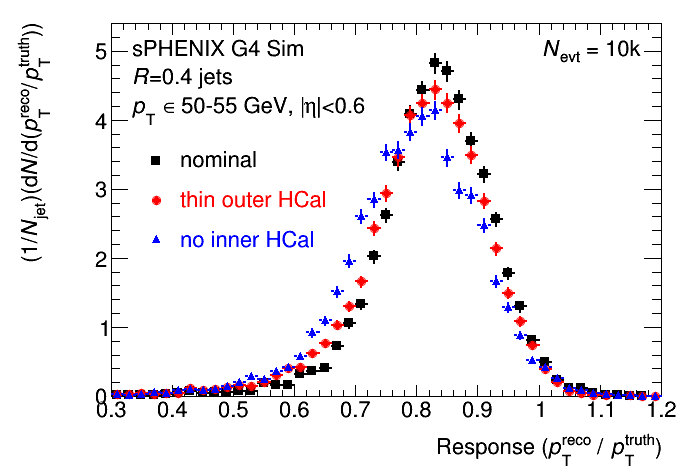
\includegraphics[width=0.4\linewidth]{figs/jetresponse_thinhcal}
  \hspace{0.1\linewidth}
  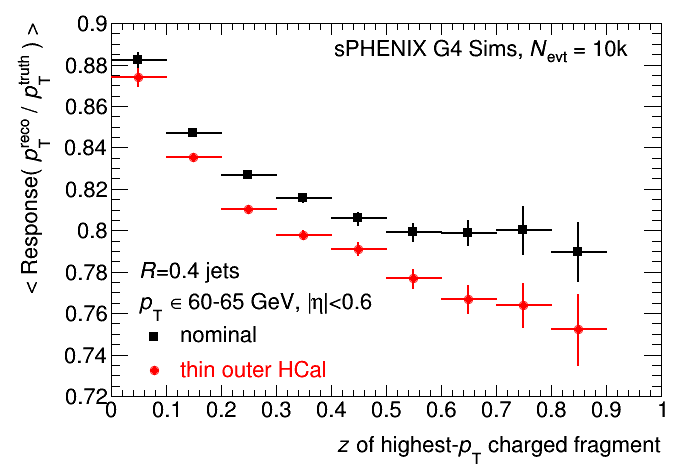
\includegraphics[width=0.4\linewidth]{figs/fragmentation_bias_thinhcal}
  \caption{(Left) Comparison of the jet response for three different HCal configurations: Nominal outer HCal (black markers), 
   outer HCal thinned by 20~cm (red markers) and no inner HCal (blue markers). 
   (Right) Comparison of the jet fragmentation bias for nominal (black markers) and thinned outer HCal (240~cm outer radius, red markers).}
  \label{fig:jet_energy_scale_thin_hcal}
\end{figure}
\paragraph{Jet energy scale}
Figure~\ref{fig:jet_energy_scale_thin_hcal}(left) shows the energy response, $p_T^{reco}/p_T^{truth}$, 
of the calorimeter system to high \pT jets for 
three calorimeter configurations: the nominal outer HCal thickness (outer radius = 260~cm), an outer HCal thinned by about one 
interaction length (outer radius = 240~cm) and nominal outer HCal and EMCal, but no inner HCal (blue markers). The simulations 
show only a small loss in total energy containment of FIXME \% for the thinned outer HCal configuration relative to the nominal
configuration, combined with a moderate increase in the number of jets for which less than 70\% of the energy was reconstructed.
Further studies showed that the change in the jet response only has a small effect on reconstructing unfolded jet spectra,
even when uing a Gaussian kernel that ignores the increases low-energy tail. Removing the inner HCal has a significantly larger
effect on the mean and shape of the jet response.

\paragraph{Fragmentation function bias} 
One expects that the thinned HCal configuration leads to the biggest change in jet response for jets with high-z fragmentation products that
are not contained in the calorimeter system. To study this effect, we plot the average jet energy response 
$\langle p_T^{reco}/p_T^{truth}\rangle$ as a function of the momentum fraction $z$ carried by the highest \pt charged (FIXME) 
fragment in Fig.\ref{fig:jet_energy_scale_thin_hcal}(right). Even for the nominal HCal configuration, a dependence of the response on the hardness of the jet fragmentation
is seen, with a change of about 0.08 in $\langle p_T^{reco}/p_T^{truth}\rangle$ from softest to hardest fragmenting jets. 
For the thinned HCal configuration, this increases to 0.11-0.13. We expect that this additional bias would only lead to a moderate 
increase in the uncertainty of fragmentation function ratios for Au+Au/p+p, as the increase is only about 50\% of the 
bias already seen in the nominal configuration, and present in both p+p and Au+Au events (i.e., only related to the 
single particle containment). 


\subsection{Outer HCal shortening}

For the shortened outer HCal (reducing the pseudorapidity coverage from $\| \eta \| <$ FIXME to $\| \eta \| < $ FIXME), all measured
at the outer corner of the calorimeter) the expected impact 
is in the statistics of jet related probes. The FIXME\% reduction in coverage will predominantly affect lower \pt jets ($\pt <$ FIXME),
as jets at the highest \pT have a narrow rapidity distribution that falls within the remaining acceptance. 
\begin{figure}[hbt]
  \centering
  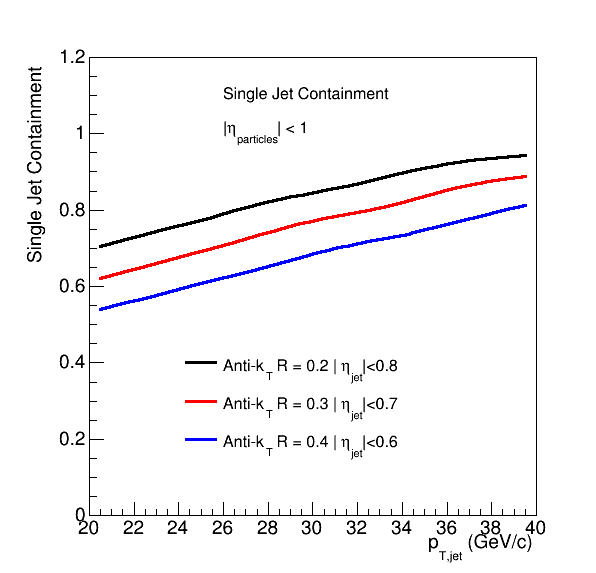
\includegraphics[width=0.4\linewidth]{figs/SingleJet_eta_reference}
  \hspace{0.1\linewidth}
  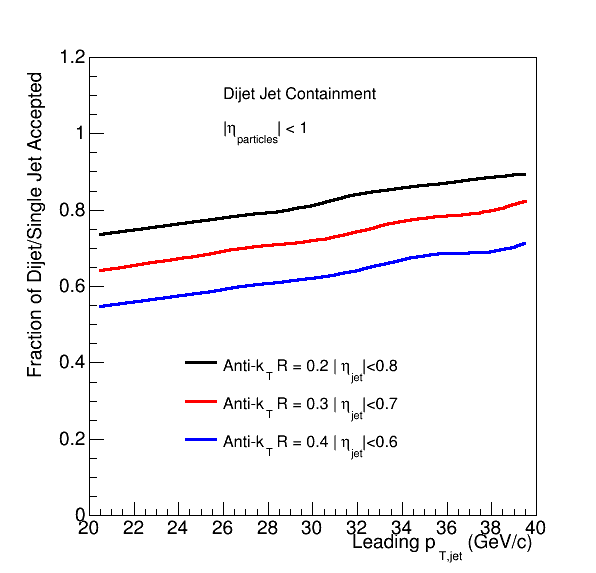
\includegraphics[width=0.4\linewidth]{figs/Dijet_eta_reference}
  \caption{(Left) 
  Fraction of jets fully contained within the acceptance of the nominal calorimeter system as a function
  of jet \pt, for three different jet radius parameters, R = 0.2 (black), R=0.3 (red) and R=0.4 (black). 
   (Right) 
  Fraction of dijets with both jets fully contained within the acceptance of the nominal calorimeter system as a function
  of jet \pt, for three different jet radius parameters, R = 0.2 (black), R=0.3 (red) and R=0.4 (black).}
  \label{fig:jet_containment_nominal}
\end{figure}
Figure~\ref{fig:jet_containment_nominal} shows the fraction of jets (left) and dijets (right) contained in the nominal calorimeter 
system as a function of jet \pt, obtained from generator level distributions. As expected, the fraction of fully contained jets is lowest for low \pT jets (which have a wider
rapidity distribution) than for hight \pt jets. The difference between the nominal length outer HCal and the shortened outer HCal
is well approximated by the difference between the black and blue curves shown in the figures.

Some of the physics impact can be recovered using tracker + EMCal reconstruction of jets, although reduced control over the jet 
energy scale and increased jet-by-jet fluctuations will limit the precision that can be achieved with such studies.

\subsection{Removal of the inner HCal}

As shown in Fig.\ref{fig:jet_energy_scale_thin_hcal}(left), the impact on jet energy scale and fluctuations for this option is 
found to be significantly larger than for the thinned outer HCal option. 
with major impact on engineering of the inner detector mechanical design leading to expectations of minimal overall savings.
We therefore did not perform detailed studies of this option.

\section{EMCal}
\subsection{Changing EMCal segmentation}
\subsubsection{2$\times$2 ganging of EMCal channels}
The reduced EMCal segmentation from 2x2 ganging of readout channels is expected to affect three physics areas: jet finding 
and jet energy reconstruction, electron/hadron separation for the $\Upsilon$ to $e^+ e^-$ channel and photon identification.
We performed full \geant and reconstruction studies of the effect on the single jet response and full \geant simulations for 
Au+Au HIJING events for electron identification. Studies of the effect on photon identification are ongoing.

\paragraph{Effect on jet energy response}
\begin{figure}[hbt]
  \centering
  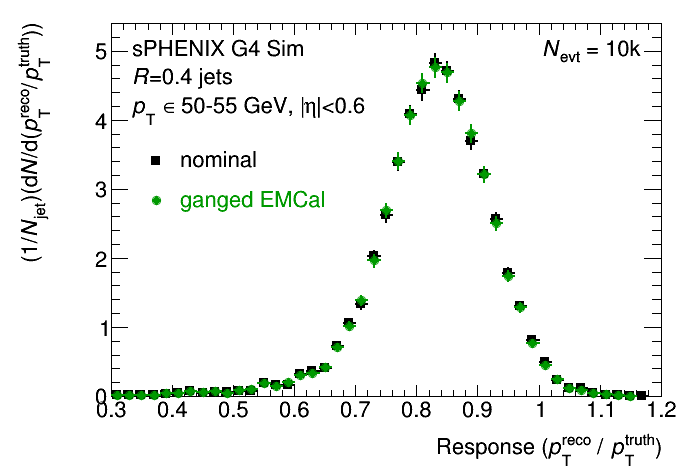
\includegraphics[width=0.4\linewidth]{figs/jetresponse_ganged_ecal}
  \hspace{0.1\linewidth}
  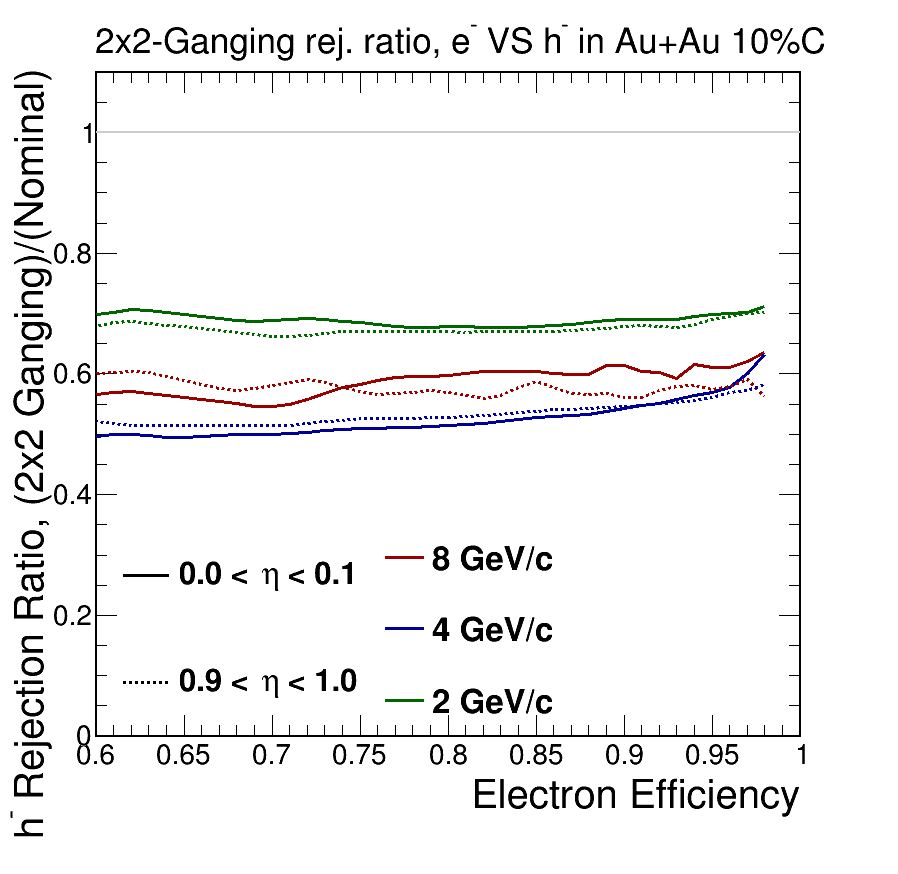
\includegraphics[width=0.4\linewidth]{figs/hadron_rejection_ganged_over_nominal}
  \caption{(Left)
  Jet response for the nominal calorimeter systems (black markers) and the calorimeter system with ganged EMCal readout 
(green markers) for high \pt jets.
   (Right)
  Ratio of the hadron rejection factor as a function of electron efficiency between the ganged EMCal configuration 
and the nominal EMCal configuration, for central Au+Au collisions. The ratio is shown for two pseudorapidity regions 
and three particle momenta. }
  \label{fig:jet_containment_nominal}
\end{figure}
Figure~\ref{fig:jet_containment_nominal}(left) shows the energy response in the calorimeter system for high \pt jets for the 
nominal configuration (black markers) and the ganged EMCal configuration (green markers). Ganging has no visible effect
on this distribution, as the change in granularity is small compared to the typical jet size and the total collected
jet and background energies are unchanged.

\begin{figure}[hbt]
  \centering
  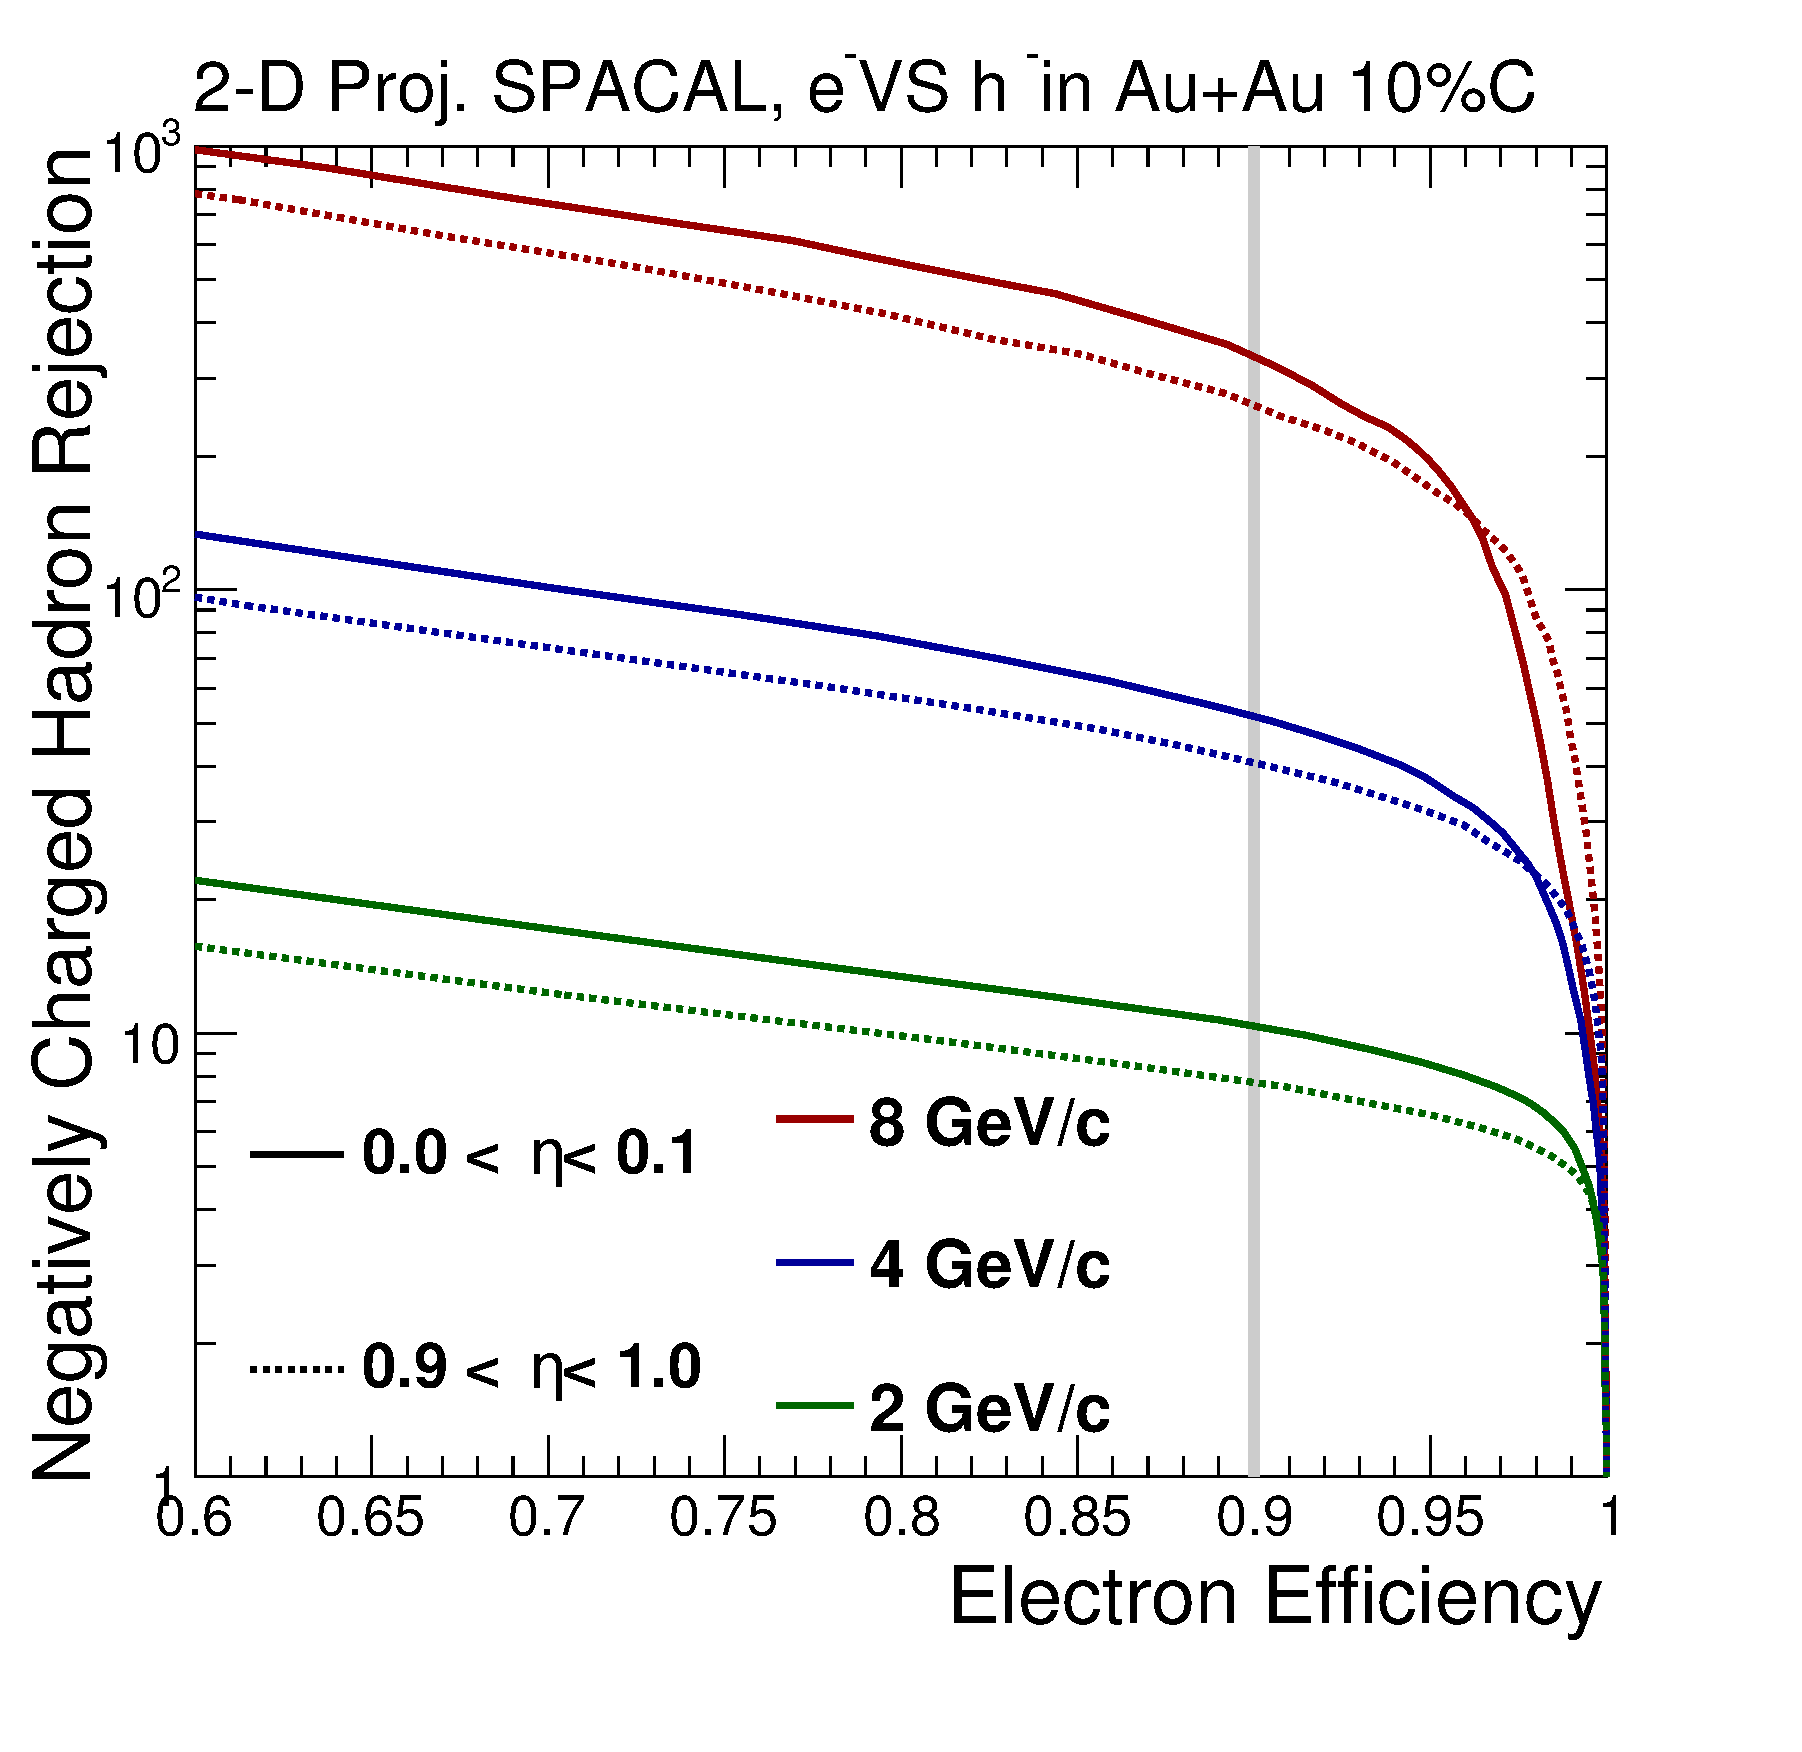
\includegraphics[width=0.4\linewidth]{figs/DrawEcal_Likelihood_Sum_RejectionCurve_AuAuSummary}
  \hspace{0.1\linewidth}
  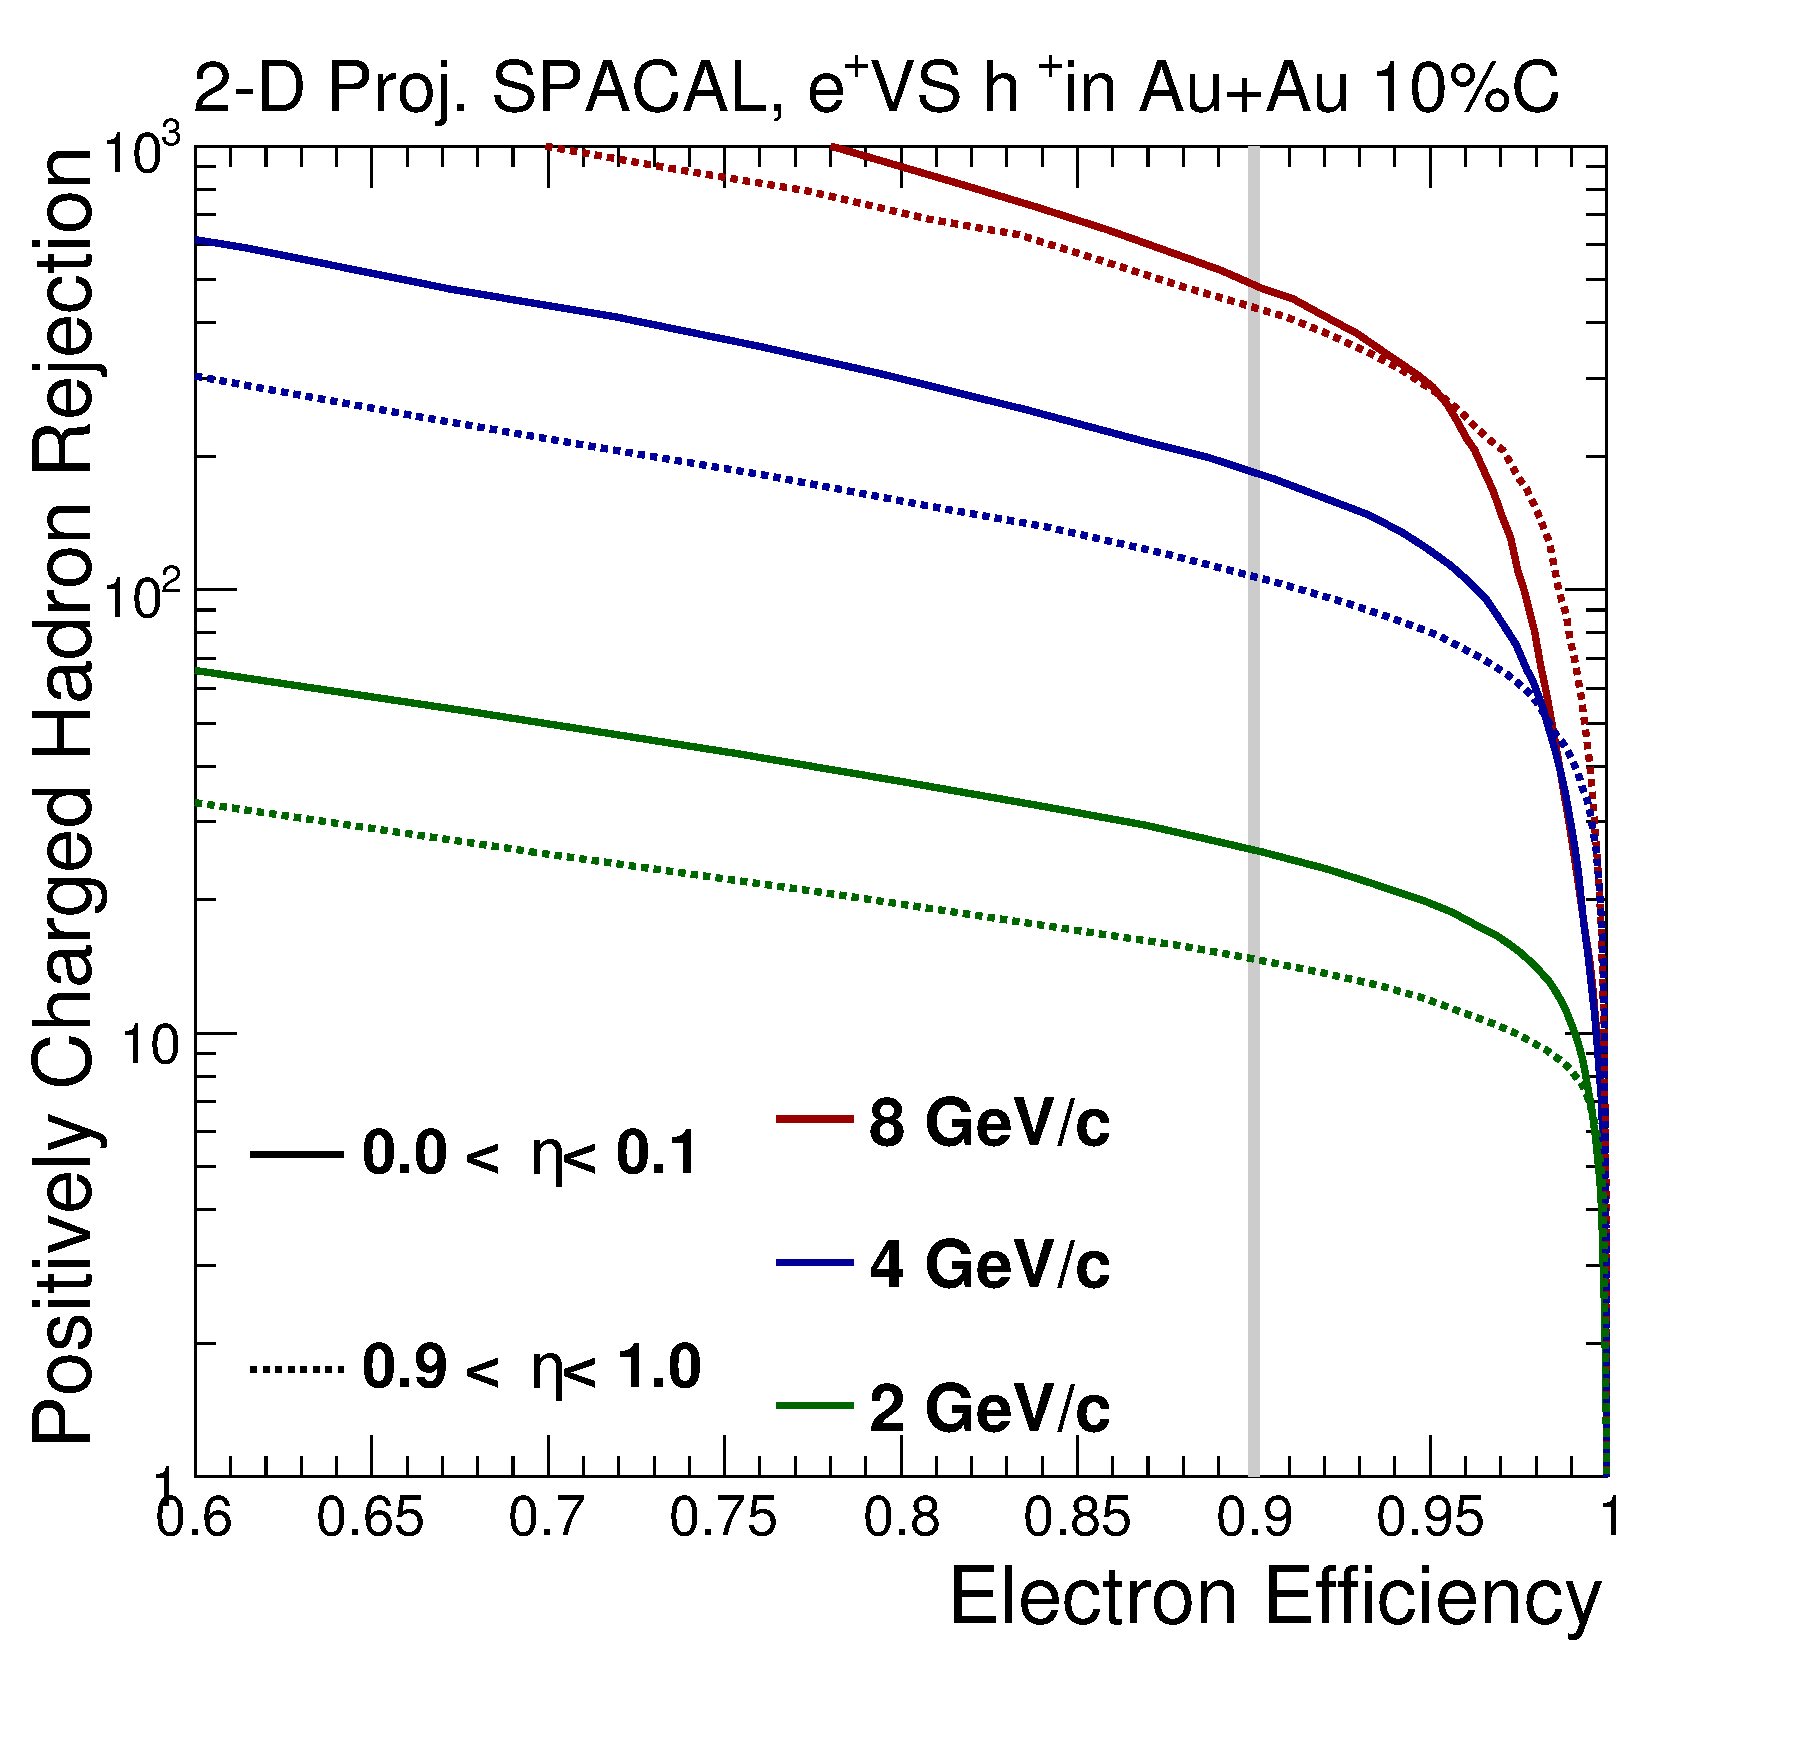
\includegraphics[width=0.4\linewidth]{figs/DrawEcal_Likelihood_Sum_RejectionCurve_AuAuSummaryPos}
  \caption{For a $2\times2$ ganged EMCal (with inner HCal present)
    inclusive charged hadron rejection is plotted on the left (right)
    as function of electron ID efficiency, for negatively (positively)
    charged tracks of three choices of momentum and for middle and
    edge rapidity in 10\% most central Au+Au events.}
  \label{fig:eid_auau}
\end{figure}

\paragraph{Effect electron/hadron separation}

The hadron rejection factors  for the $2\times 2$ EMCal readout ganging where obtained for HIJING simulations of central Au+Au collisions, and are
shown for negative (left) and positive (right) hadrons as a function of electron efficiency in Fig.~\ref{fig:eid_auau}. 
The relative change compared to simulations of the nominal EMCal configuration can be seen in Fig.~\ref{fig:jet_containment_nominal}(right), which shows
the ratio of the hadron rejection factor between the ganged configuration and the nominal configuration as a function
of electron efficiency for central Au+Au collisions. The change in rejection factor ranges from the 0.7 for low \pt hadrons
at central rapidity to 0.5 for intermediate \pt hadrons at central rapidity. Simulations of the current nominal EMCal 
configuration show a rejection factor of about 200 for the kinematic range relevant for $\Upsilon$ identification at FIXME\%
electron efficiency. The rejection factor for the nominal configuration is twice as large as that assumed (FIXME) 
for $\Upsilon$ studies in the pCDR. The loss in rejection by a factor of two for the ganged configuration is significant, but
will still allow the $\Upsilon$ program as discussed in the pCDR, albeit with a reduced safety margin.

\subsubsection{Increasing EMCal tower size}
The reduced EMCal segmentation from increasing the tower dimensions
from $d\eta \times d\phi = 0.024 \times 0.024$ to $0.033 \times 0.28$
was not evaluated with full \geant simulations, as time did not permit
implementing the corresponding detector geometry. However, as the
change increases the tower area by 60\%, as compared to a factor of
four for the 2x2 ganging, the expected impact can be well estimated
based on the 2x2 ganging full simulations. For the jet response, the
2x2 ganging did not show any noticable effect, implying that the 60\%
increased tower size will also have no effect on jets. For $e/h$
separation, the effect of the 2x2 ganging of about a factor of two
suggests scaling with the $\sqrt{\mbox{area}}$, i.e., the fluctuations
in the background energy. This implies a 26\% change (FIXME) in
$e/\pi$ separation in central Au+Au collisions for the 60\% increase
in tower size, which is well within the projected safety margin for
the measurement.

\subsection{Reduced EMCal pseudorapidity coverage}
Reducing the EMCal coverage to $\| \eta \| < 0.6$ will directly affect
the expected statistics for $\Upsilon$ to $e^+ e^-$ and photon-based
measurements. The corresponding loss in statistics is summarized in
the table below, based on generator level studies. For jet
measurements, the reduced coverage leads to a change in jet response
across the EMCal boundary. This effect was evaluated by full \geant
simulations and reconstruction of the single jet response in different
regions of pseudorapidity and jet \pt.

\paragraph{Loss of $\Upsilon$ acceptance}
\begin{figure}[hbt]
  \centering
  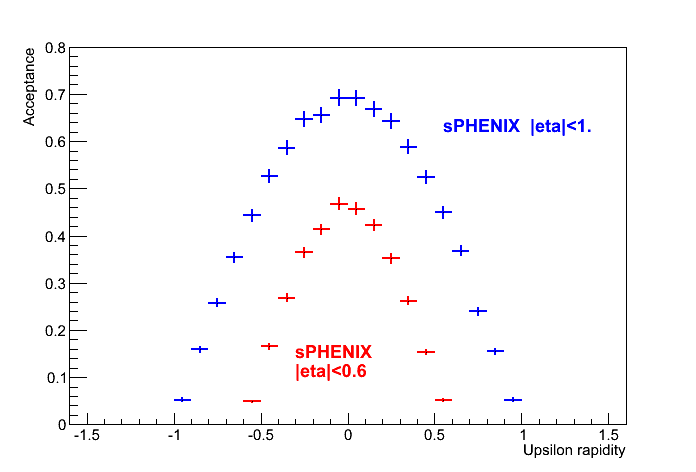
\includegraphics[width=0.4\linewidth]{figs/upsilon_rate_y}
  \hspace{0.1\linewidth}
  \includegraphics[width=0.4\linewidth]{figs/upsilon_rate_pT}
  \caption{(Left)
  $\Upsilon$ to $e^+ e^-$ acceptance as a function of rapidity for the nominal (blue markers) and $\| \eta \| < 0.6$ configurations,
  averaged over $\Upsilon$ \pt. 
  (Right) $\Upsilon$ to $e^+ e^-$ acceptance as a function of $\pt$ for the nominal (blue markers) and $\| \eta \| < 0.6$ 
  configurations, averaged over $\eta$.}
  \label{fig:upsilon_rate}
\end{figure}

Figure~\ref{fig:upsilon_rate} shows the acceptance for $\Upsilon$ to $e^+ e^-$ decays for the nominal and reduced $\eta$ EMCal
configurations as a function of rapidity (left) and $\pt$ (right). The figures suggest a loss of about 60\% of overall 
$\Upsilon$ statistics, with the largest effect at low \pt. In $\Upsilon$ rapidity, about 0.5 units in rapidity reach are 
lost when requiring equal $\Upsilon$ statistics for nominal and reduced $\eta$ configurations.

\paragraph{Change in jet response} 
\begin{figure}[hbt]
  \centering
  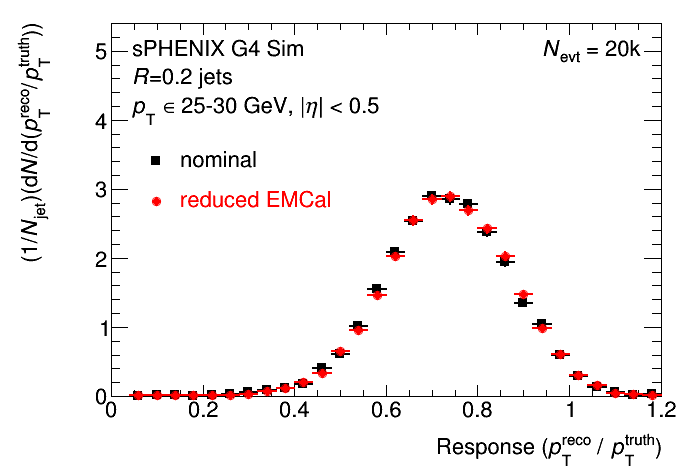
\includegraphics[width=0.4\linewidth]{figs/jet_response_reduced_emcal_eta_0} 
  \hspace{0.1\linewidth}
  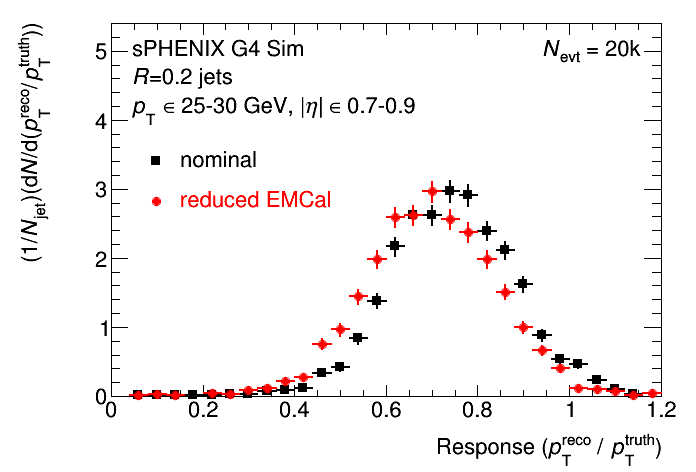
\includegraphics[width=0.4\linewidth]{figs/jet_response_reduced_emcal_eta_07}
  \caption{(Left) Comparison of jet response for $|\eta|$ < 0.5 jets for nominal (black markers) and reduced acceptance (red markers) EMCal configuration.
  (Right) Comparison of jet response for $|\eta|$ > 0.5 jets for nominal (black markers) and reduced acceptance (red markers) EMCal configuration.}
  \label{fig:jet_response_reduced_emcal}
\end{figure}

The effect of reducing the EMCal acceptance to $|\eta| < 0.6$ on the jet energy response, $p_T^{reco}/p_T^{truth}$, was studied
for low \pt jets, where we expect the largest effect, for three regions of jet pseudorapidity, $|\eta| < 0.5$ (Fig.\ref{fig:jet_response_reduced_emcal}, left), $0.5 < |\eta| < 0.7$ (not shown) and $|\eta| > 0.7$ (Fig.\ref{fig:jet_response_reduced_emcal}, right). As expected, essentially no change
is observed for the central rapidity region. For $0.5 < |\eta| < 0.7$, the jet energy response shifts by FIXME \%, while for $|\eta| > 0.7$ a 
shift of FIXME \% is seen, as well as an enhance low response tail. Experience at LHC suggest typical best-case jet response uncertainties
of 2-3\%. Assuming an uncertainty in the correction of the reduced response at large $\eta$ of 50\% or better, the changed response
compared to the nominal configuration will lead to a significant, but still tolerable increase in unfolding uncertainties for jet spectra.

\begin{figure}[hbt]
  \centering
  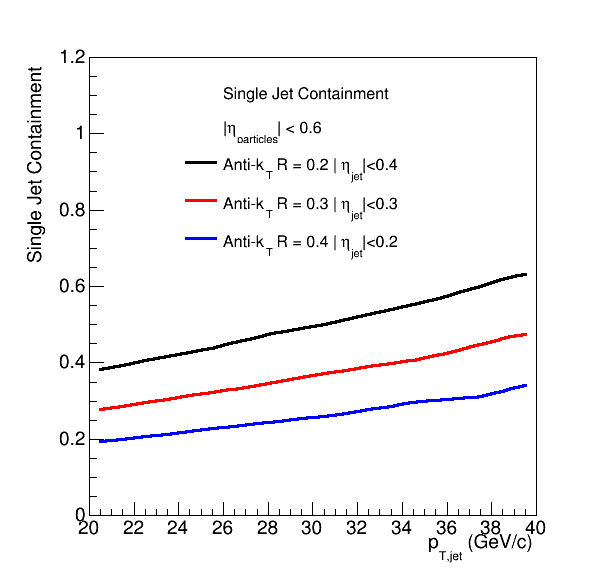
\includegraphics[width=0.4\linewidth]{figs/SingleJet_eta_ecal06}
  \hspace{0.1\linewidth}  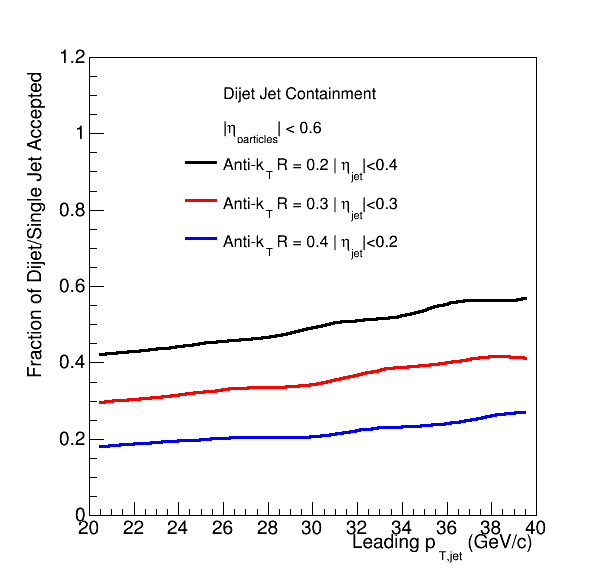
\includegraphics[width=0.4\linewidth]{figs/Dijet_eta_ecal06}
  \caption{(Left)
  Fraction of jets fully contained within the acceptance of the $|\eta| < 0.6$ EMCal configuration as a function
  of jet \pt, for three different jet radius parameters, R = 0.2 (black), R=0.3 (red) and R=0.4 (black).
   (Right)
  Fraction of dijets with both jets fully contained within the acceptance of $|\eta| < 0.6$ configuration as a function
  of jet \pt, for three different jet radius parameters, R = 0.2 (black), R=0.3 (red) and R=0.4 (black).}
  \label{fig:jet_containment_reduced_emcal}
\end{figure}

We also investigated the loss in statistics when requiring jets and dijets to be fully contained in the reduced EMCal acceptance. The result is shown 
in Fig.\ref{fig:jet_containment_reduced_emcal}, to be compared with the acceptance for the nominal 
configuration shown in Fig.~\ref{fig:jet_containment_nominal}. One observes that for low \pt dijets, this requirement leads to a loss of dijet
statistics by a factor of 2-3, depending on the selected jet radius parameter $R$.

\section{Outer tracker}

For the outer tracker, the performance of a TPC tracker was evaluated using \geant simulations of single particles, single $\Upsilon$ to $e^+ e^-$
decays, and full HIJING and \geant simulations in a limited acceptance around mid-rapidity (due to timing limitations). Simulations were performed
for an ideal TPC and two configurations with inner field cage boundary at $r=20$~cm and $r=30$~cm. For the latter configurations, effects of 
residual space charge distortions expected after corrections were included. We evaluated general performance characteristics (efficency, fake track
rate, DCA and momentum resolution) and specifically the $\Upsilon$ mass resolutions for the different cases. The TPC simulations were performed
in combination with the 3-layer MAPS configuration of the reference design, and include the effects of track reconstruction and kinematic fits. 
The effect of various inner tracker options on the tracking performance is evaluated separately in \ref{sec:innertracker}.

\subsection{Studies of $\Upsilon$ mass resolution}

We have performed TPC simulations with and without residual space charge distortions
(i.e., after corrections)  and for readout of 60 and 30 TPC layers, for a field cage configuration with 20~cm inner radius and 78~cm outer radius 
in all cases. The space charge distortions are calculated follow the prescriptions outlined in the ALICE TDR and 
specifically the results from the thesis of Rossiger.  We use a second order Langevin equation to 
swim particles through the static electric and magnetic fields producing a pair of distortion results $dr(r,z)$ and $rd{\phi}(r,z)$.  
Our calculations are normalized to ALICE gas conditions (Ne, CO2 90:10) and reproduce well the distortion in the ALICE TDR.  

For simplicity, we have assumed that post-correction errors due to space charge distortions will be linearly proportional to the amount of the 
distortion itself.  These errors are modeled as two portions, labelled as "accuracy" and "precision".  Errors in accuracy will move points 
in a correlated fashion due to either over- or under-correcting the distortion.  In meetings with ALICE, they quoted a 1 mm accuracy 
after a correction of 20 cm.  Errors in precision are due to fluctuations in the instantaneous space charge distribution as compared to the average.  
ALICE projects that through great effort (new space charge patterns every 5 msec) they will correct a 20 cm distortion to 200 microns while STAR currently corrects a 10 cm distortion to 400 microns.  Our calculations have used "precisionFactors" of 0.001 (ALICE), 0.004 (STAR), and 0.010 (worse than either).

Table~\ref{tab:upsilon_mass_resolution} summarizes the outcome of these simulations for the FIXME precisionFactor. Reducing the number of 
read out TPC layers from 60 to 30 yields an increase in $\Upsilon$ mass resolution by about 10~MeV, still well within the resolution required
for a separation of the three $\Upsilon$ states. The smaller dimensions of the sPHENIX TPC compared to e.g., ALICE and the change of the inner
field cage radius to $r = 20$~cm, which moves the largest distortions out of the sensitive volume, yield much smaller distortions expected
for sPHENIX than those seen/expected in ALICE and STAR. After correction, the effect of residual distortions on the $\Upsilon$ mass resolution is 
found to be on the order of 1~MeV.

\begin{table}
  \centering
  \begin{tabular}{lr}
    \toprule
    Configuration & $\Upsilon$ mass resolution \\
    \midrule
3 maps layers and 60 TPC layers with no distortion due to space charge
&  66 MeV/$c^2$ \\
3 maps layers and 30 TPC layers with no distortion due to space charge
& 76 MeV/$c^2$ \\
3 maps layers and 60 TPC layers with distortions due to space charge
& 67.4 MeV/$c^2$ \\
3 maps layers and 30 TPC layers with distortions due to space charge
& 77.2 MeV/$c^2$ \\
    \bottomrule
  \end{tabular}
  \caption{Effects of corrected TPC space charge distortions and sparsified readout on the $\Upsilon$ mass resolution.}
  \label{tab:upsilon_mass_resolution}
\end{table}



\section{Inner tracker}
\label{sec:innertracker}

To isolate the effect of various inner tracker configurations, simulations for central Au+Au HIJING events were performed for 
combinations of an ``ideal'' outer tracker consisting of a 4-layer configuration of MAPS sensors in cylinder geometry and 
3 inner tracker configurations:
\begin{itemize}
\item A three-layer MAPS configuraton based on the ALICE ITS IB detector (``reference'')
\item A two-layer MAPS configuraton corresponding to the two innermost (?? FIXME) layers of ALICE ITS IB detector
\item A two-layer detector configuraton based on re-used pixel ladders from the PHENIX VTX detector, using ladders with
the least known dead areas. 
\end{itemize}

The performance of the 3-layer reference inner tracker can be seen in Fig.~\ref{fig:tracking_reference}, showing the 
transverse momentum resolution, $d\pt/\pt$, (left), the DCA resolution with respect to the primary vertex (center) 
and track finding efficiency (right), all as a function of true particle \pt for central HIJING Au+Au collisions. 
\begin{figure}[hbt]
  \centering
  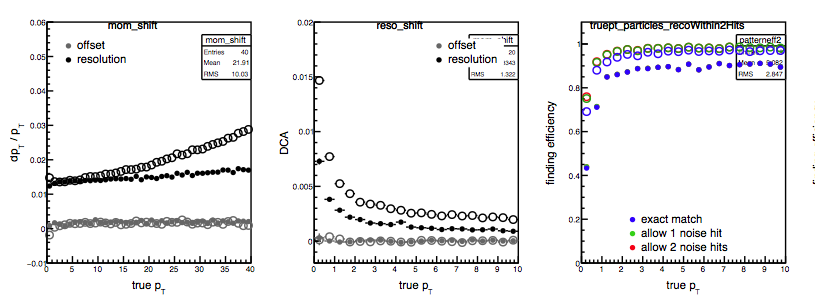
\includegraphics[width=0.9\linewidth]{figs/tracking_performance_reference}
  \caption{Tracking performance for the reference detector configuration with an
  outer TPC tracker and a 3-layer MAPS inner tracker. Shown are \pt resolution (left), 
  DCA resolution with respect to the primary vertex (center) and track finding efficiency (right), all as a function
of true particle \pt for central HIJING Au+Au collisions.}
  \label{fig:tracking_reference}
\end{figure}

\subsection{VTX pixel configuration} FIXME - add same plot as \ref{fig:tracking_reference}, but replacing the 3-layer MAPS with the VTX pixel 
configuration
\subsection{2-layer MAPS tracker} FIXME - add same plot as \ref{fig:tracking_reference}, but replacing the 3-layer MAPS with a two-layer MAPS configuration
configuration

\section{DAQ and trigger}
\subsection{Minimum bias trigger counter and vertex locator}
We expect that the proposed re-use of an existing vertex detector, or the potential copy of the STAR EPD under construction, will not significantly affect
the physics performance for any of the benchmark measurements.
\subsection{Offline event building}
We expect that the proposed change of event-building strategy will not significantly affect the physics performance for any of the benchmark measurements,
although it will likely introduce an additional latency in the initial offline reconstruction that remains to be evaluated.

\section{Interference of calorimeter options}
Most of the re-scoping options discussed in this document can be considered independently and combined to achieve certain levels of savings 
and physics performance. This is not the case when considering combinations of some of the HCAL and EMCal options with respect to the 
jet reconstruction performance. This includes in particular:
\begin{itemize}
\item Thinning of the outer HCAl by $\approx 20$~cm
\item Removal of the inner HCal
\item Reduction of the EMCal acceptance to $|\eta| < 0.6$
\end{itemize}
Each of these options in essence removes about one interaction length from the calorimeter system. Our simulations show that for a 
change by one interaction length the resulting change in calorimeter response is significant, but not dominant compared to the typical
systematic uncertainties achieved in such measurements. Combining two such changes in the same acceptance region however leads to 
a degradation in energy containment that significantly degrades performance. An example of this is shown for the combined effect of 
outer HCAL thinning and reduced EMCal acceptance in Fig.~\ref{fig:JetResponse25GeV_CaloStackVariants_Nevt20k_ETABIN2}. While the
performance compared to the nominal configuration is acceptable for either the thinned outer HCal (blue) or the reduced acceptance EMCal,
the combination of both changes, shown as green markers, leads to a jet energy response with a most likely ratio of $p_T^{reco}/p_T^{truth} 
\approx 0.3$ and a wide tail. Experience at LHC suggest that it is unlikely that such a response function could be unfolded with sufficient accuracy
to yield high precision jet spectra. In essence, the options listed above are mutually exclusive when aiming for accurate jet energy
measurements.

\begin{figure}[hbt]
  \centering
  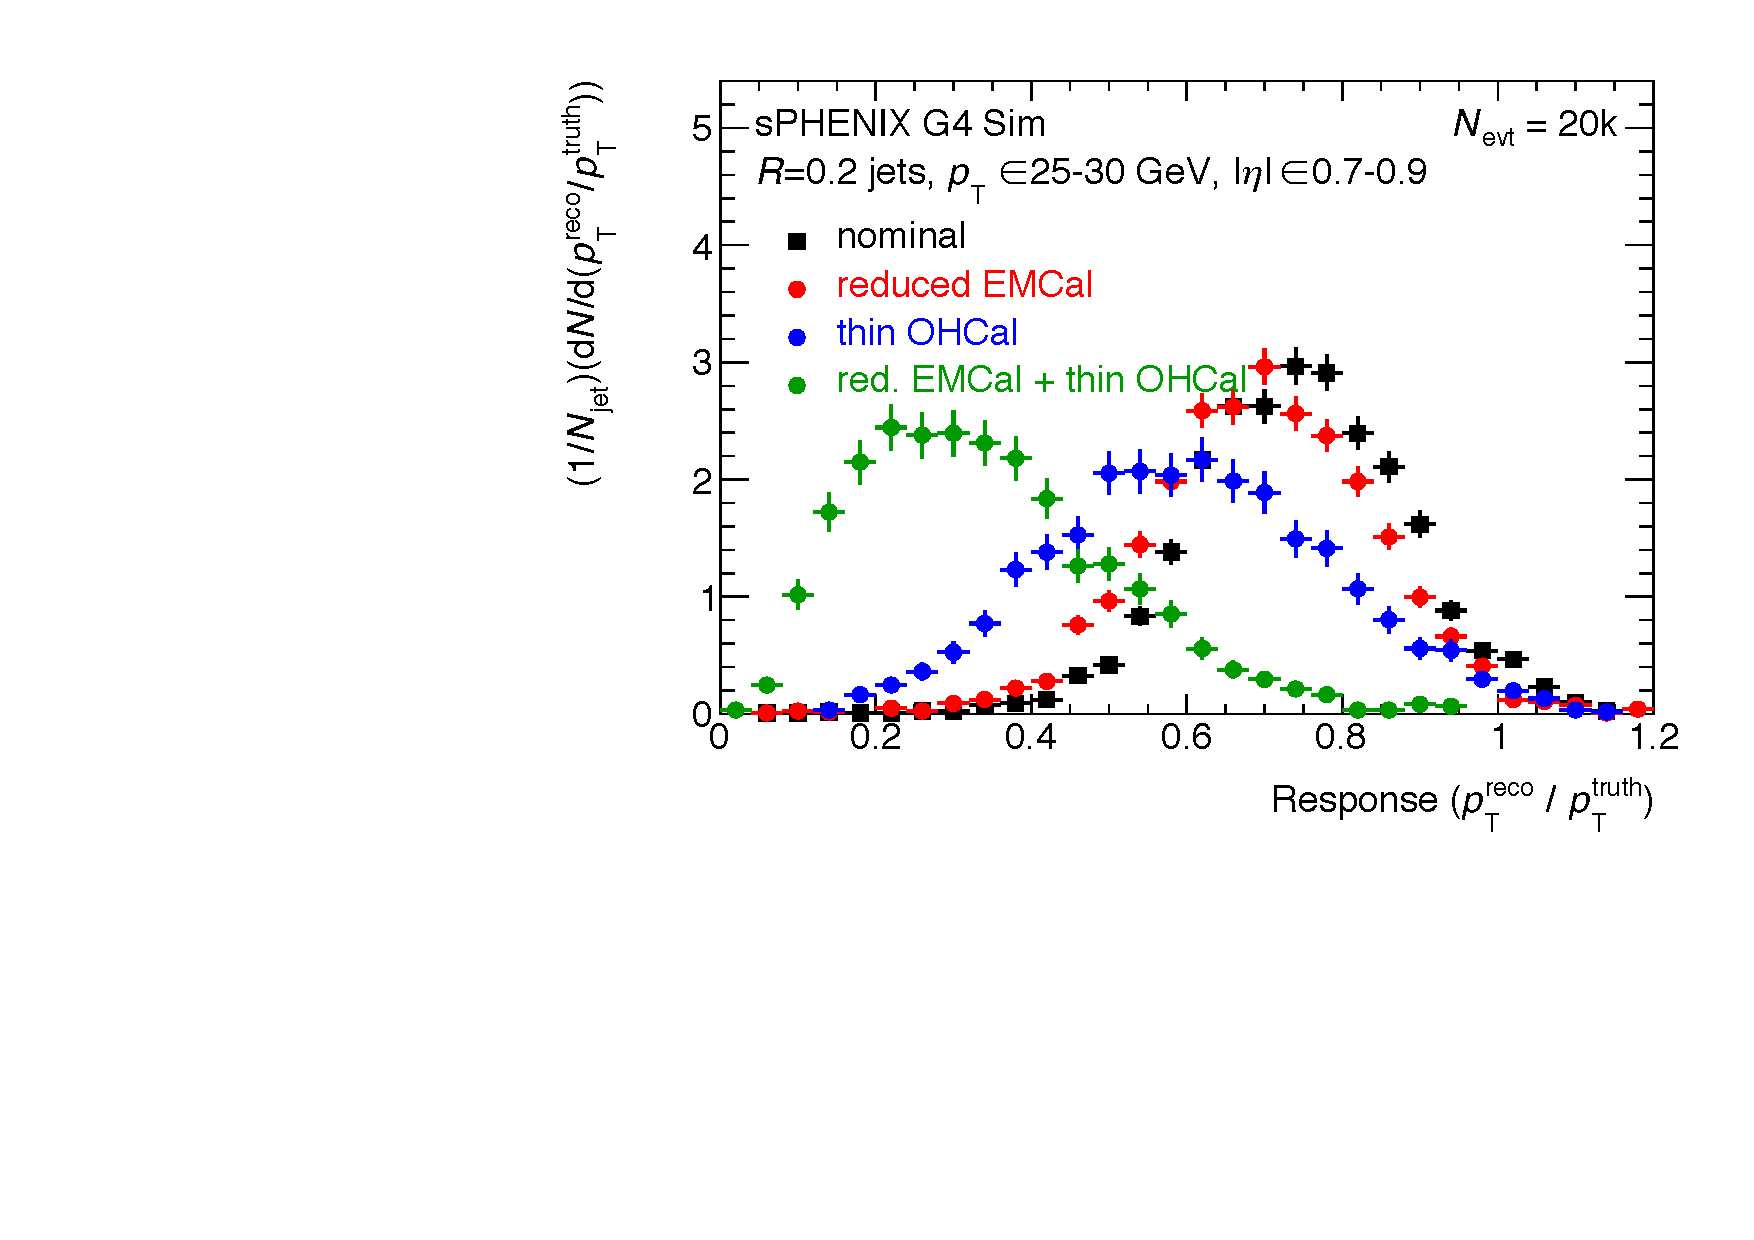
\includegraphics[width=0.9\linewidth]{figs/sPHENIX_JetResponse25GeV_CaloStackVariants_Nevt20k_ETABIN2}
  \caption{Jet response for low \pt jets at forward $|\eta| > 0.7$ for four calorimeter configurations:
   nominal (black markers), reduced EMCal acceptance (red), thinned outer HCAL (blue) and a combination
   reduced acceptance EMCal and thinned outer HCal (green markers).}
  \label{fig:JetResponse25GeV_CaloStackVariants_Nevt20k_ETABIN2}
\end{figure}






\chapter*{Charge}
\label{charge}

\begin{figure}[hbt!]
  \centering
  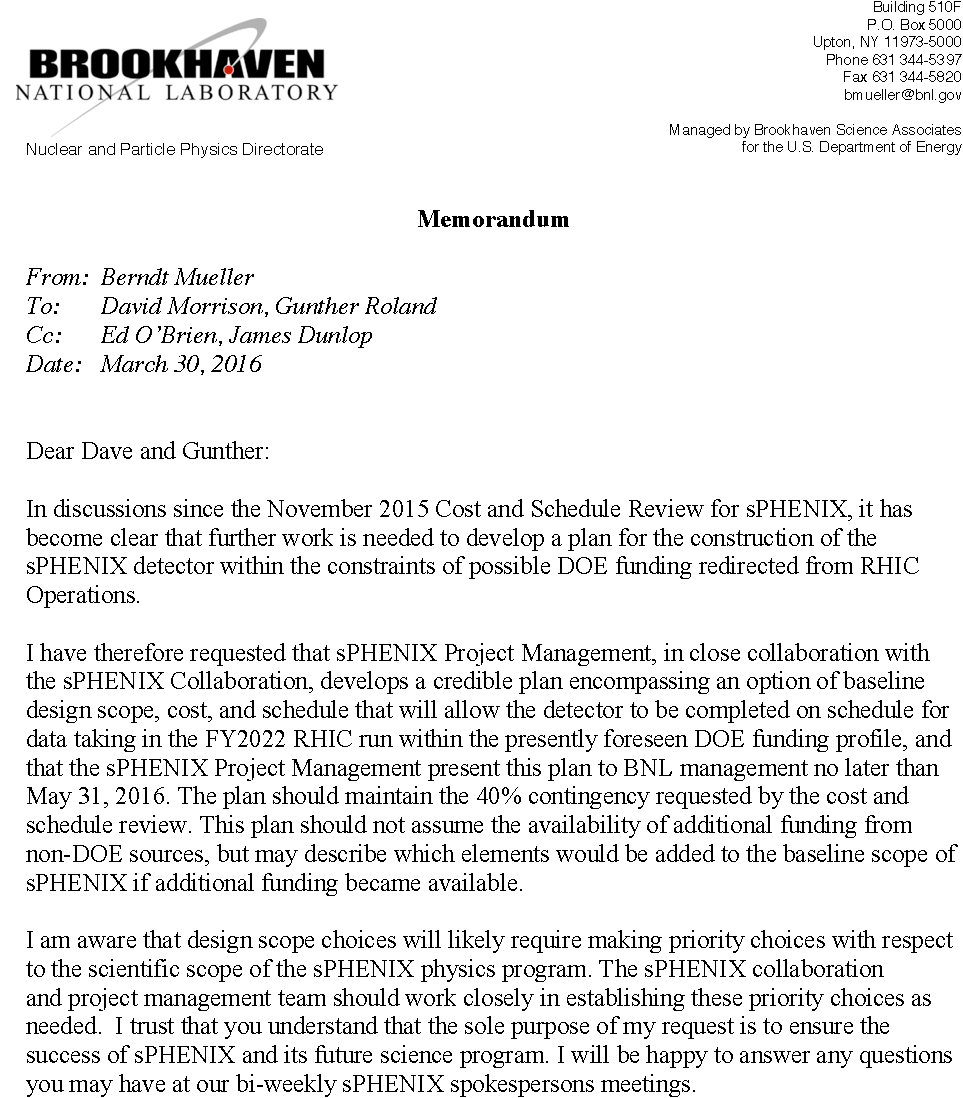
\includegraphics[width=0.8\linewidth]{charge_memo}
\end{figure}



\cleardoublepage

\backmatter

\cleardoublepage
\phantomsection
\addcontentsline{toc}{chapter}{List of Tables}
%\listoftables

\cleardoublepage
\phantomsection
\addcontentsline{toc}{chapter}{List of Figures}
%\listoffigures

\cleardoublepage
\phantomsection
%\addcontentsline{toc}{chapter}{References}

%\bibliographystyle{unsrturl}
%\bibliography{refs}

\end{document} 


